\documentclass[conference]{IEEEtran}

\usepackage{tikz}
\usepackage{cite}
\usepackage{caption}
\usepackage{algorithm}
\usepackage[noend]{algpseudocode}


\usepackage[slovene]{babel}

% correct bad hyphenation here
\hyphenation{}

\begin{document}
	
	\title{Ekstrakcija podatkov}
	
	\author{Skupina \textbf{DOMACI-NJOKI}: Niki Bizjak, Bojan Vrangeloski, Uroš Škrjanc}
	
	\maketitle
	
	\begin{abstract}
		Cilj prve seminarske naloge je bil napisati pajka, ki zna s spleta prenašati spletne vsebine in jih shranjevati v podatkovno bazo. Pred iskanjem podatkov po taki podatkovni bazi, pa je treba prenesene vsebine najprej prečistiti in iz njih izluščiti pomembne informacije. V drugem seminarju si bomo ogledali tri različne načine za ekstrakcijo podatkov iz HTML vsebin.
	\end{abstract}
	
	\IEEEpeerreviewmaketitle
	
	\section{Uvod}
	
	Druga seminarska naloga pri predmetu Iskanje in ekstrakcija podatkov s spleta je namenjena pridobivanju informacij iz vsebin, ki jih je s spleta prenesel pajek. V seminarju smo si ogledali tri različne načine ekstrakcije - dva taka, ki zahtevata veliko uporabnikovega poseganja in razumevanja strukture strani in tretjega, ki zna informacije prepoznati in izluščiti avtomatično, s primerjavo podobnih spletnih strani.
	
	Ekstrakcijo podatkov smo izvajali na štirih različnih spletnih straneh, ki jih glede na strukturo razdelimo na dve skupini:
	
	\begin{itemize}
		\itemsep 0em
		\item \textbf{list} - stran vsebuje \textit{seznam} izdelkov, artiklov, člankov, ipd.
		\item \textbf{detail} - stran prikazuje podatke za en izdelek, članek, ipd.
	\end{itemize}

	Tabela \ref{tab:tipi}, prikazuje naše testne strani, razvrščene glede na tipa strani, opisana zgoraj.
	
	\begin{table}[h]
		\centering
		\begin{tabular}{l|l}
			Stran & Tip \\ 
			\hline 
			\texttt{overstock.com} & list \\ 
			\texttt{rtvslo.si} & detail \\ 
			\texttt{bolha.com} & list \\ 
			\texttt{avto.net} & detail \\ 
		\end{tabular}
		\caption{Tip strani za posamezno domeno, nad katero smo izvajali ekstrakcijo podatkov}
		\label{tab:tipi}
	\end{table}
	
	\section{Regularni izrazi}
	
	Regularni izrazi nam omogočajo učinkovito iskanje informacij v nizih z uporabo končnih avtomatov. Regularni izrazi se lahko uporabijo za preverjanje, če posamezen niz vsebuje iskan vzorec. Pri implementaciji ekstrakcije z regularnimi izrazi, smo si pomagali s vgrajeno Python knjižnico \texttt{re}. 
	
	Za ekstrakcijo podatkov s strani Overstock, smo uporabili regularne izraze, prikazane na sliki \ref{fig:overstock-regex}. Najprej smo za vsako iskano polje na strani definirali svoj regularni izraz, nato pa smo jih z ustreznimi vmesnimi regularnimi izrazi, povezali v skupen izraz, ki zna hkrati poiskati vse podatke. Na podoben način smo ekstrahirali podatke tudi iz ostalih spletnih strani. Regularne izraze za spletno stran RTV SLO lahko vidimo na sliki \ref{fig:rtvslo-regex}, slika \ref{fig:avtonet-regex}, pa prikazuje regularne izraze za spletno stran \texttt{Avto.net}.
	
	\begin{figure}
		\centering
		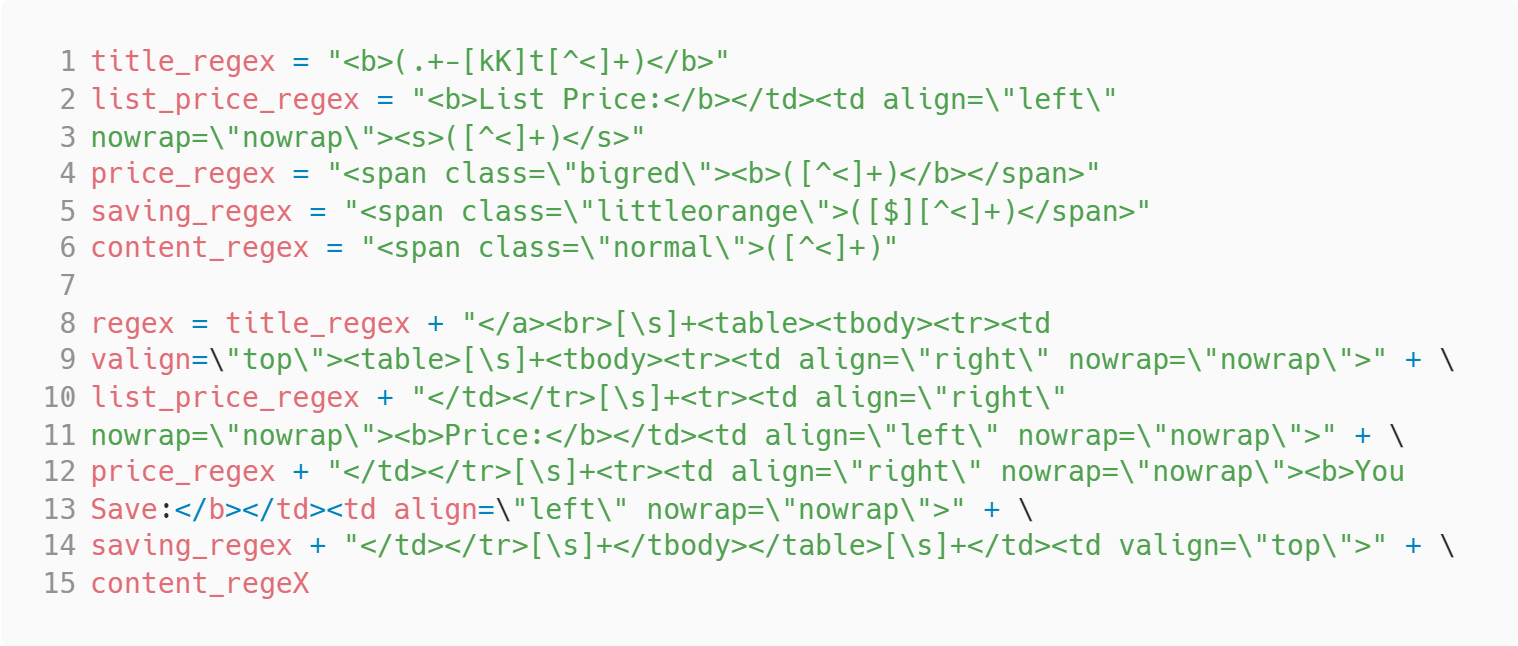
\includegraphics[width=0.9\linewidth]{images/overstock_regex}
		\caption{Regularni izrazi, uporabljeni za ekstrakcijo podatkov s strani Overstock}
		\label{fig:overstock-regex}
	\end{figure}

	\begin{figure}
		\centering
		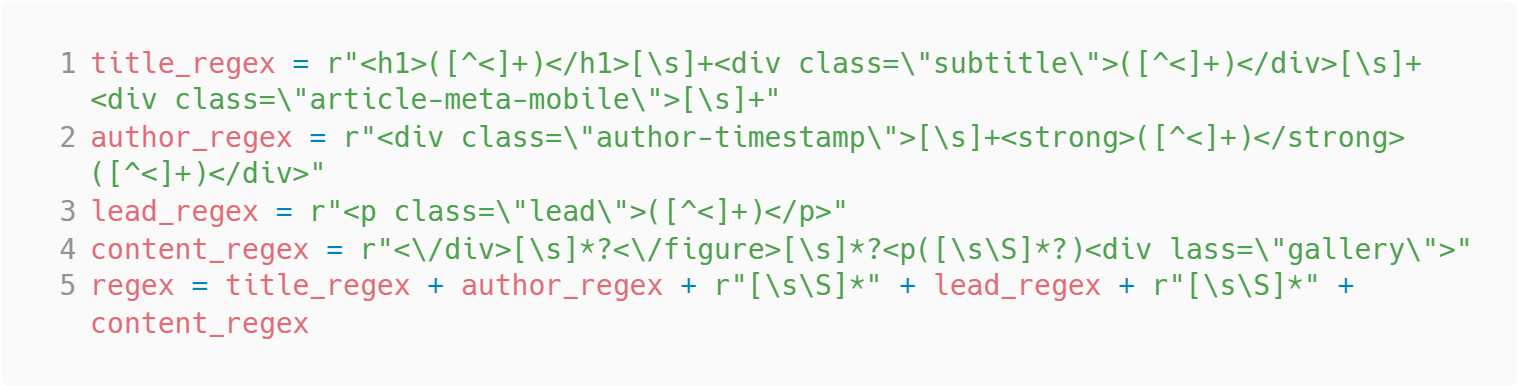
\includegraphics[width=0.9\linewidth]{images/rtvslo_regex}
		\caption{Regularni izrazi, uporabljeni za ekstrakcijo podatkov s strani RTV SLO}
		\label{fig:rtvslo-regex}
	\end{figure}

	\begin{figure}
		\centering
		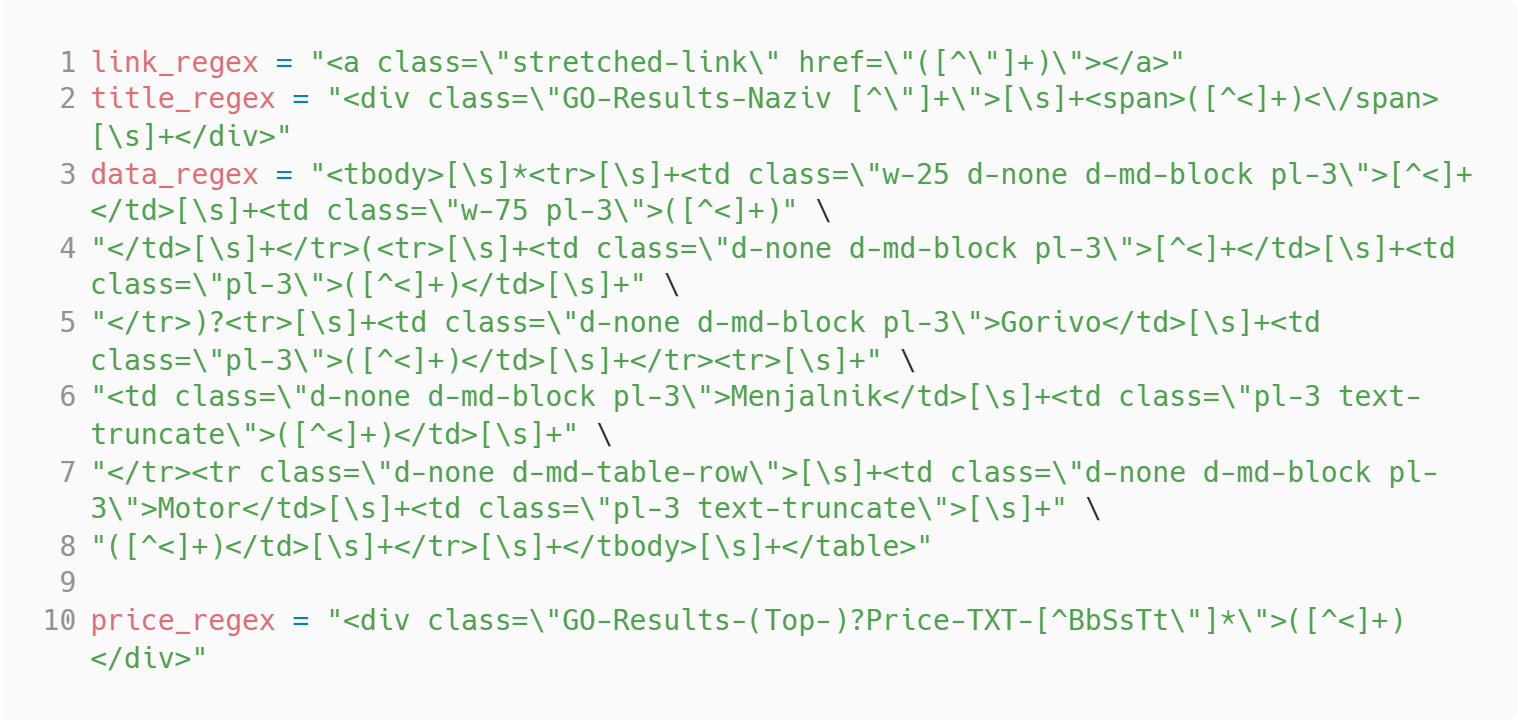
\includegraphics[width=0.9\linewidth]{images/avtonet_regex}
		\caption{Regularni izrazi, uporabljeni za ekstrakcijo podatkov s strani Avto.net}
		\label{fig:avtonet-regex}
	\end{figure}

	\section{XPath}
	
	XPath je poizvedovalni jezik, ki je bil razvit za namene ekstrakcije podatkov iz XML podatkovnih struktur. Izrazi so sestavljeni v obliki datotečnih poti in lahko vsebujejo pogoje za spust po določeni veji drevesa, klice funkcij nad vejami, ipd. Slike \ref{fig:overstock-xpath}, \ref{fig:rtvslo-xpath}, \ref{fig:avtonet-xpath} in \ref{fig:bolha-xpath} prikazujejo XPath izraze, ki smo jih uporabili za ekstrakcijo podatkov iz izbranih spletnih strani.
	
	Največje težave sta predstavljali strani \texttt{Avto.net} in Overstock, saj elementi niso bili semantično označeni. Ostale strani imajo namreč z razredi ali identifikatorji označene elemente na strani, kar olajša iskanje, saj lahko take elemente hitro najdemo s filtriranjem. Spletna stran Overstock je sestavljena iz vgnezdenih tabel, kar še posebej oteži iskanje, saj je potrebno poznati indekse elementov, ki jih iščemo. Če se taka stran le malo spremeni, bi naši XPath izrazi ne delovali več.
	
	\begin{figure}
		\centering
		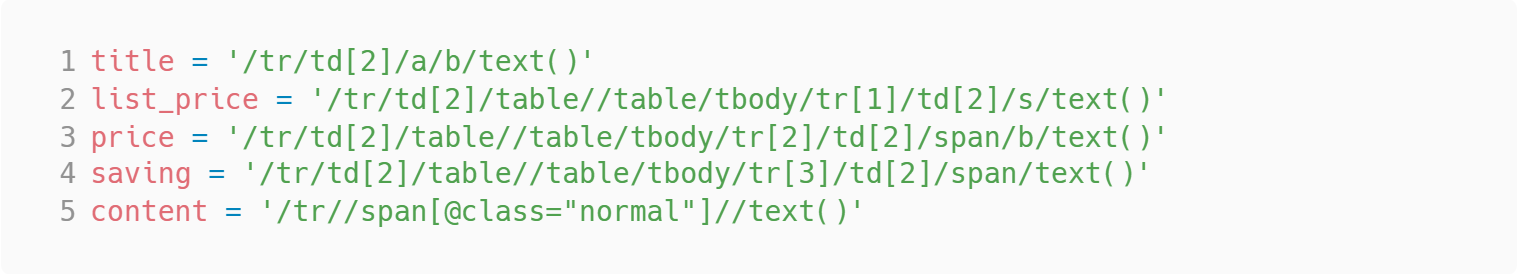
\includegraphics[width=0.9\linewidth]{images/overstock_xpath}
		\caption{XPath izrazi, uporabljeni za ekstrakcijo podatkov s strani Overstock}
		\label{fig:overstock-xpath}
	\end{figure}

	\begin{figure}
		\centering
		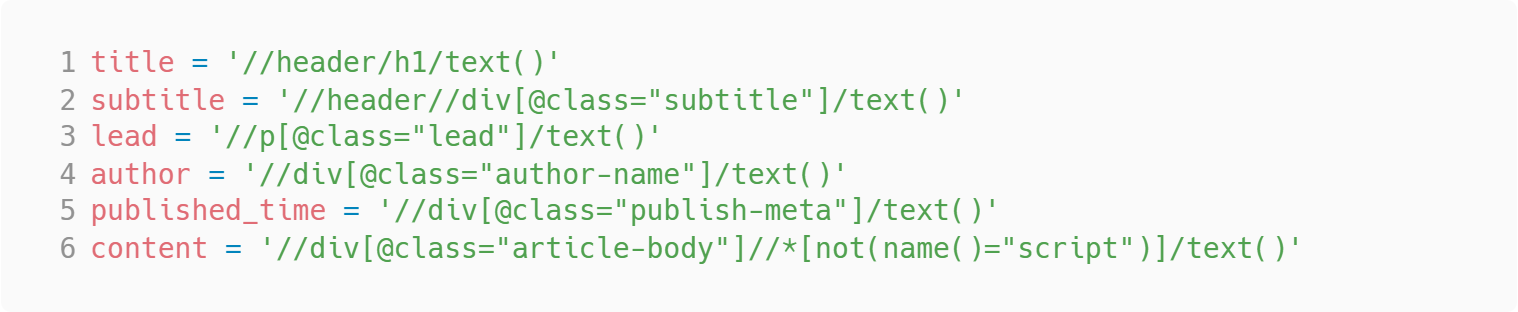
\includegraphics[width=0.9\linewidth]{images/rtvslo_xpath}
		\caption{XPath izrazi, uporabljeni za ekstrakcijo podatkov s strani RTV SLO}
		\label{fig:rtvslo-xpath}
	\end{figure}

	\begin{figure}
		\centering
		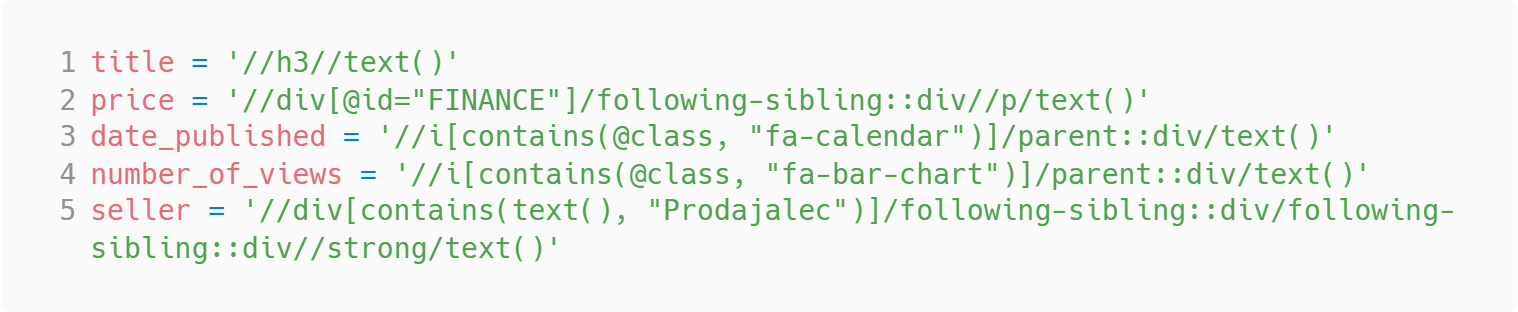
\includegraphics[width=0.9\linewidth]{images/avtonet_xpath}
		\caption{XPath izrazi, uporabljeni za ekstrakcijo podatkov s strani Avto.net}
		\label{fig:avtonet-xpath}
	\end{figure}

	\begin{figure}
		\centering
		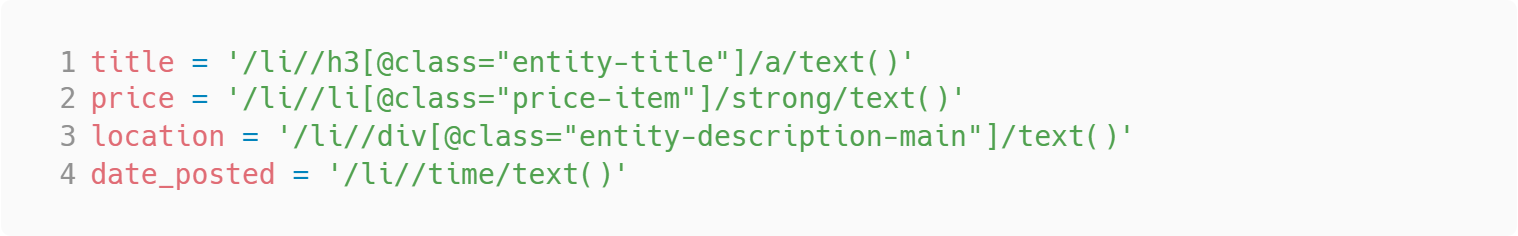
\includegraphics[width=0.9\linewidth]{images/bolha_xpath}
		\caption{XPath izrazi, uporabljeni za ekstrakcijo podatkov s strani Bolha}
		\label{fig:bolha-xpath}
	\end{figure}
	
	\section{Avtomatična ekstrakcija podatkov}
	
	Na spletu se od uvedbe programskega jezika PHP naprej pojavlja dosti dinamičnih spletnih strani. Take strani hranijo podatke v podatkovni bazi in glede na dostopan URL naslov izvedejo poizvedbo v podatkovni bazi in na podlagi rezultata prikažejo podatke v uporabniku prijazni obliki. Pri avtomatični ekstrakciji podatkov, bi radi na podlagi dveh strani, ki imata enako strukturo, a drugačno vsebino, zgradili program, ki zna samodejno pridobiti podatke.
	
	V našem primeru smo za avtomatično ekstrakcijo podatkov uporabili algoritem \textsc{RoadRunner}~\cite{roadrunner, crescenzi2001automatic}. Ta sicer v originalni implementaciji deluje na seznamu žetonov (angl. token), v našem primeru pa smo za predstavitev HTML vsebin uporabili kar DOM drevo. Algoritem deluje tako, da v pomnilnik prebere dve datoteki - ovojnico (angl. wrapper) in drugi dokument. S pomočjo funkcije \textsc{Generalize}, skuša nato ovojnico ustrezno uskladiti z dokumentom tako, da išče istoležne elemente, v njih išče polja (angl. fields) in opcijske elemente (angl. optionals).
	
	Implementiran algoritem zna na strani prepoznati polja, tj. elemente, ki se pojavijo na obeh straneh, a imajo drugačne vrednosti. Prav tako zna program prepoznati opcijske elemente, tj. elemente, ki se pojavijo v enem izmed dokumentov, v drugem pa ne. Našo implementacijo bi lahko izboljšali tako, da bi dodali prepoznavanje iteratorjev, tj. elementov, ki se ponavljajo. Tega dela nam zaradi pomanjkanja časa, ni uspelo implementirati.
	
%	\begin{algorithm}
%		\caption{Generalizacija ovojnice}\label{octree}
%		\begin{algorithmic}[1]
%			\Procedure{Generalize}{wrapper, document}
%				\If{(wrapper is text) and (document is text)}
%					\State We have discovered a field
%					\State Replace wrapper text with \texttt{\#PCDATA}
%				\Else
%					\If {\textsc{Tag}(wrapper) $\neq$ \textsc{Tag}(document)}
%						\State This is a tag mismatch, end
%					\Else
%						
%					\EndIf
%				\EndIf
%			\EndProcedure
%		\end{algorithmic}
%	\end{algorithm}
	
	\section{Zaključek}
	
	Pisanje regularnih in XPath izrazov za pridobivanje podatkov je zamudno in od razvijalca zahteva poznavanje oziroma razumevanje strukture spletne strani. Kljub temu, pa daje tak način ekstrakcije podatkov boljše rezultate, saj podatke označimo oziroma umestimo v nek kontekst. Razvijalec lahko npr. na mestih kjer se pojavijo cela števila, le-ta iz nizov pretvori v številčno predstavitev in s tem še dodatno opiše podatke. Avtomatična ekstrakcija podatkov je princip, pri katerem sistem na strani sam najde polja, ki vsebujejo podatke. Rezultati, tj. neoznačene izluščene informacije pa so v tem primeru pogosto pomanjkljivi oziroma težko razumljivi.
	
	Prva metoda je uporabna predvsem v primerih, ko je potrebno izluščiti podatke iz ene same spletne strani. Pisanje izrazov je časovno potratno in je smiselno, kadar vemo, da se bo struktura spletne strani spreminjala zelo redko.
	
	Druga metoda je zelo uporabna v primeru, ko imamo za ekstrahirati podatke iz ogromne količine različnih strani in smo za prihranek časa, pripravljeni žrtvovati natančnost.
	
	\bibliographystyle{IEEEtran}
	\bibliography{bibliography}
	
\end{document}
